% Options for packages loaded elsewhere
\PassOptionsToPackage{unicode}{hyperref}
\PassOptionsToPackage{hyphens}{url}
\documentclass[
  11pt,
]{article}
\usepackage{xcolor}
\usepackage[left=3cm,right=3cm,top=2.5cm,bottom=2.5cm]{geometry}
\usepackage{amsmath,amssymb}
\setcounter{secnumdepth}{5}
\usepackage{iftex}
\ifPDFTeX
  \usepackage[T1]{fontenc}
  \usepackage[utf8]{inputenc}
  \usepackage{textcomp} % provide euro and other symbols
\else % if luatex or xetex
  \usepackage{unicode-math} % this also loads fontspec
  \defaultfontfeatures{Scale=MatchLowercase}
  \defaultfontfeatures[\rmfamily]{Ligatures=TeX,Scale=1}
\fi
\usepackage{lmodern}
\ifPDFTeX\else
  % xetex/luatex font selection
\fi
% Use upquote if available, for straight quotes in verbatim environments
\IfFileExists{upquote.sty}{\usepackage{upquote}}{}
\IfFileExists{microtype.sty}{% use microtype if available
  \usepackage[]{microtype}
  \UseMicrotypeSet[protrusion]{basicmath} % disable protrusion for tt fonts
}{}
\usepackage{setspace}
\makeatletter
\@ifundefined{KOMAClassName}{% if non-KOMA class
  \IfFileExists{parskip.sty}{%
    \usepackage{parskip}
  }{% else
    \setlength{\parindent}{0pt}
    \setlength{\parskip}{6pt plus 2pt minus 1pt}}
}{% if KOMA class
  \KOMAoptions{parskip=half}}
\makeatother
\usepackage{longtable,booktabs,array}
\usepackage{caption}
\captionsetup[table]{skip=6pt}
\newcounter{none} % for unnumbered tables
\usepackage{calc} % for calculating minipage widths
% Correct order of tables after \paragraph or \subparagraph
\usepackage{etoolbox}
\makeatletter
\patchcmd\longtable{\par}{\if@noskipsec\mbox{}\fi\par}{}{}
\makeatother
% Allow footnotes in longtable head/foot
\IfFileExists{footnotehyper.sty}{\usepackage{footnotehyper}}{\usepackage{footnote}}
\makesavenoteenv{longtable}
\usepackage{graphicx}
\makeatletter
\newsavebox\pandoc@box
\newcommand*\pandocbounded[1]{% scales image to fit in text height/width
  \sbox\pandoc@box{#1}%
  \Gscale@div\@tempa{\textheight}{\dimexpr\ht\pandoc@box+\dp\pandoc@box\relax}%
  \Gscale@div\@tempb{\linewidth}{\wd\pandoc@box}%
  \ifdim\@tempb\p@<\@tempa\p@\let\@tempa\@tempb\fi% select the smaller of both
  \ifdim\@tempa\p@<\p@\scalebox{\@tempa}{\usebox\pandoc@box}%
  \else\usebox{\pandoc@box}%
  \fi%
}
% Set default figure placement to htbp
\def\fps@figure{htbp}
\makeatother
% definitions for citeproc citations
\NewDocumentCommand\citeproctext{}{}
\NewDocumentCommand\citeproc{mm}{%
  \begingroup\def\citeproctext{#2}\cite{#1}\endgroup}
\makeatletter
 % allow citations to break across lines
 \let\@cite@ofmt\@firstofone
 % avoid brackets around text for \cite:
 \def\@biblabel#1{}
 \def\@cite#1#2{{#1\if@tempswa , #2\fi}}
\makeatother
\newlength{\cslhangindent}
\setlength{\cslhangindent}{1.5em}
\newlength{\csllabelwidth}
\setlength{\csllabelwidth}{3em}
\newenvironment{CSLReferences}[2] % #1 hanging-indent, #2 entry-spacing
 {\begin{list}{}{%
  \setlength{\itemindent}{0pt}
  \setlength{\leftmargin}{0pt}
  \setlength{\parsep}{0pt}
  % turn on hanging indent if param 1 is 1
  \ifodd #1
   \setlength{\leftmargin}{\cslhangindent}
   \setlength{\itemindent}{-1\cslhangindent}
  \fi
  % set entry spacing
  \setlength{\itemsep}{#2\baselineskip}}}
 {\end{list}}
\usepackage{calc}
\newcommand{\CSLBlock}[1]{\hfill\break\parbox[t]{\linewidth}{\strut\ignorespaces#1\strut}}
\newcommand{\CSLLeftMargin}[1]{\parbox[t]{\csllabelwidth}{\strut#1\strut}}
\newcommand{\CSLRightInline}[1]{\parbox[t]{\linewidth - \csllabelwidth}{\strut#1\strut}}
\newcommand{\CSLIndent}[1]{\hspace{\cslhangindent}#1}
\setlength{\emergencystretch}{3em} % prevent overfull lines
\providecommand{\tightlist}{%
  \setlength{\itemsep}{0pt}\setlength{\parskip}{0pt}}
%% tools/stamp.tex
%% Provenance footer for PDFs rendered from this project.
%% Vendored by zzcollab; this file is not project-specific. The
%% footer prints the source document and the time of rendering.
%% The git version is defined here too, and so is available to a
%% project that wants it on the page, but it is left off the
%% default footer: it already names the staged copy in share/ and
%% appears in its manifest row. All values are supplied at render
%% time by tools/stamp-render.R, which writes a small generated
%% file that redefines the macros below. The \providecommand
%% defaults keep a bare LaTeX compile working when the document is
%% built without the wrapper.
\usepackage{fancyhdr}
\usepackage{xcolor}
\providecommand{\stampsource}{\detokenize{(source not recorded)}}
\providecommand{\stamptime}{(time not recorded)}
\providecommand{\stampversion}{\detokenize{(version not recorded)}}
\setlength{\footskip}{40pt}
\newcommand{\stampfootcontent}{%
  \footnotesize\color{gray}%
  \parbox[b]{\textwidth}{%
    \stamptime\hfill\thepage\\[2pt]%
    \ttfamily\raggedright\stampsource}}
\pagestyle{fancy}
\fancyhf{}
\fancyfoot[C]{\stampfootcontent}
\renewcommand{\headrulewidth}{0pt}
\renewcommand{\footrulewidth}{0.4pt}
%% The title page uses the `plain` page style; redefine it so the
%% stamp appears there too.
\fancypagestyle{plain}{%
  \fancyhf{}%
  \fancyfoot[C]{\stampfootcontent}%
  \renewcommand{\headrulewidth}{0pt}%
  \renewcommand{\footrulewidth}{0.4pt}}
\renewcommand{\stampsource}{\textasciitilde{}/\allowbreak{}prj/\allowbreak{}res/\allowbreak{}18-mmrm-vs-lm-simple/\allowbreak{}mmrmlm/\allowbreak{}analysis/\allowbreak{}report/\allowbreak{}report.Rmd}
\renewcommand{\stamptime}{2026-08-20 13:51 PDT}
\renewcommand{\stampversion}{\detokenize{a2220a1-wip}}
\usepackage{amsmath}
\usepackage{amssymb}
\usepackage{booktabs}
\usepackage{longtable}
\usepackage{float}
\usepackage[mathlines]{lineno}
\linenumbers
\usepackage{placeins}
\usepackage{bm}
\usepackage{booktabs}
\usepackage{longtable}
\usepackage{array}
\usepackage{multirow}
\usepackage{wrapfig}
\usepackage{float}
\usepackage{colortbl}
\usepackage{pdflscape}
\usepackage{tabu}
\usepackage{threeparttable}
\usepackage{threeparttablex}
\usepackage[normalem]{ulem}
\usepackage{makecell}
\usepackage{xcolor}
\usepackage{bookmark}
\IfFileExists{xurl.sty}{\usepackage{xurl}}{} % add URL line breaks if available
\urlstyle{same}
% fallback for those not using the hyperref driver hyperxmp:
\makeatletter
\@ifundefined{xmpquote}{\newcommand{\xmpquote}[1]{#1}}{}
\makeatother
\hypersetup{
  pdftitle={When Do Random Effects Models Reduce to Fixed-Effect Alternatives? Conditions for Equivalence in Longitudinal Clinical Trials},
  pdfauthor={Ronald G. Thomas, Ph.D.},
  hidelinks,
  pdfcreator={LaTeX via pandoc}}

\title{When Do Random Effects Models Reduce to Fixed-Effect Alternatives? Conditions for Equivalence in Longitudinal Clinical Trials}
\author{Ronald G. Thomas, Ph.D.\thanks{Wertheim School of Public Health, UCSD; ORCID: 0000-0003-1686-4965}}
\date{August 20, 2026}

\begin{document}
\maketitle
\begin{abstract}
Mixed models for repeated measures (MMRM) are the default
primary analysis for continuous longitudinal endpoints in
clinical trials, but their variance-component machinery is
often opaque to collaborators. We synthesize and verify, by
Monte Carlo simulation, two settings in which a random-effects
or joint model reduces to a simpler fixed-effect analysis. In
a two-timepoint pre-post design with complete data, an
unstructured-covariance MMRM and an ANCOVA conditioning on
baseline yield algebraically identical treatment-effect point
estimates; we give a short proof and confirm it by simulation
across a \(3 \times 3\) grid of correlation and variance-ratio
values. In a three-timepoint design with a slope-only random
effect and no random intercept, a per-subject mean-change
estimator remains within half a percent of a random-slopes
linear mixed model's standard error across the full simulated
range of between-subject slope variability, a design-specific
finding we contrast with an earlier, non-reproducible version of
this simulation that reported divergence traceable to a
data-generating/fitted-model mismatch. We report both settings
under a common Wald reference distribution with Monte Carlo
standard
errors per Morris, White, and Crowther (2019), and we state
explicitly the conditions under which the simpler analysis is
exact, approximate, or inadequate. This paper does not claim new
theory; its contribution is a single accessible account, with
simulation-verified thresholds and decision guidance, for the
applied statistician deciding when the mixed-model apparatus
earns its complexity.
\end{abstract}

{
\setcounter{tocdepth}{2}
\tableofcontents
}
\setstretch{1.1}
\section{Introduction}\label{introduction}

\textbf{Keywords:} MMRM; ANCOVA; mixed models; longitudinal data;
clinical trials; equivalence; Monte Carlo simulation.

\subsection{The practical problem}\label{the-practical-problem}

In clinical trials with repeated measurements, mixed
models for repeated measures (MMRM) and random
effects models have become the standard analytic
approach\textsuperscript{\citeproc{ref-mallinckrodt2001type}{1},\citeproc{ref-mallinckrodt2008recommendations}{2}}. These models
accommodate within-subject correlation, handle
incomplete data under the missing-at-random
assumption, and provide flexible covariance
structures. However, they impose a substantial
interpretive burden on collaborators unfamiliar with
the statistical machinery of variance components,
restricted maximum likelihood estimation, and
covariance parameterization.

A natural question arises: under what conditions does
the random effects model reduce to, or closely
approximate, a simpler fixed-effect analysis that
would be more accessible to the statistical
practitioner? If such conditions can be identified,
the simpler model offers an intuitive bridge to the
same inferences, sparing the analyst from invoking
a complex apparatus when it is not strictly
necessary.

\subsection{Foundational results}\label{foundational-results}

The relationship between random effects and
fixed-effect analyses has been explored from several
angles.\textsuperscript{\citeproc{ref-brogan1980comparative}{3}} showed that in a
two-group pretest-posttest design, the
repeated-measures ANOVA subsumes the difference-score
\(t\)-test: the interaction \(F\)-statistic equals the
square of the two-sample \(t\)-test on difference
scores. The difference-score analysis requires fewer
assumptions (homogeneous variance of differences and
normally distributed errors) than the full
repeated-measures model (equal variance-covariance
matrices across groups). This algebraic embedding
demonstrates that when the research question
concerns only whether treatment groups differ in
their pre-to-post change, the simpler analysis is
not merely an approximation but is arithmetically
identical to a component of the more elaborate model.

\textsuperscript{\citeproc{ref-laird1982random}{4}} introduced the general framework
for random-effects models in longitudinal data that
has since become ubiquitous. In their formulation,
the random effects induce a structured
variance-covariance matrix on the marginal
distribution of the observed data. The key insight
for our purposes is that when this marginal
covariance is left unconstrained (as in the
unstructured covariance MMRM) the random effects
become a computational device rather than a
substantive modeling choice.

\subsection{The Frost-Kenward-Fox observation}\label{the-frost-kenward-fox-observation}

\textsuperscript{\citeproc{ref-frost2008optimizing}{5}} established a methodological
framework for comparing conventional and run-in trial
designs using linear mixed models. In their treatment
of the two-timepoint case, they showed that the
Laird-Ware random-intercept formulation treating
baseline and follow-up as correlated outcomes (their
equation 8) yields identical point estimates and very
similar standard errors to the analysis of covariance
model that conditions on baseline (their equation 6).
This near-equivalence holds provided the
variance-covariance matrix is unconstrained and
\(\sigma_{12} < \sigma_1^2\) and
\(\sigma_1^2 = \sigma_2^2\) (i.e., homogeneous marginal
variances and positive but not perfect correlation).
The result builds on\textsuperscript{\citeproc{ref-lee1974note}{6}}, who showed that
Rao's reduction of the\textsuperscript{\citeproc{ref-potthoff1964generalized}{7}}
generalized MANOVA model yields estimators identical
to those from an analysis of covariance.

\subsection{Constrained longitudinal data analysis}\label{constrained-longitudinal-data-analysis}

\textsuperscript{\citeproc{ref-liang2000longitudinal}{8}} formalized the constrained
longitudinal data analysis (cLDA), in which baseline
is included in the response vector and the model
constrains the two treatment groups to share a common
baseline mean---a consequence of randomization.\textsuperscript{\citeproc{ref-liu2009baseline}{9}} compared cLDA to the longitudinal
ANCOVA model and showed that (a) with complete data,
the treatment effect estimates are effectively
identical but the cLDA standard errors are marginally
smaller; and (b) with missing baseline data, cLDA is
more efficient because it can borrow information from
the observed outcome model to impute baseline values
implicitly under the missing-at-random assumption.\textsuperscript{\citeproc{ref-lu2009sample}{10}} derived sample-size formulae for cLDA,
and\textsuperscript{\citeproc{ref-lu2010efficiency}{11}} provided a formal efficiency
comparison of cLDA versus longitudinal ANCOVA,
quantifying the power gain as a function of the
proportion of missing baselines.

\subsection{The role of summary statistics}\label{the-role-of-summary-statistics}

An alternative thread, developed by\textsuperscript{\citeproc{ref-frison1992repeated}{12}} and\textsuperscript{\citeproc{ref-frison1997linearly}{13}},
advocates analyzing repeated measures through summary
statistics (typically the mean post-baseline value or
a fitted slope for each subject) followed by a
between-group comparison of these summaries.\textsuperscript{\citeproc{ref-senn2000repeated}{14}} extended this approach, showing that
summary-statistic methods can be viewed as special
cases of the general mixed model when the
within-subject covariance is compound symmetric.\textsuperscript{\citeproc{ref-senn2006change}{15}} provided an influential clarification
of the debate between change-score analysis and
ANCOVA, demonstrating that ANCOVA does not require
baseline balance for unbiasedness and that the common
slope assumption is testable and often reasonable.

\subsection{Modern MMRM practice}\label{modern-mmrm-practice}

In contemporary pharmaceutical practice, MMRM with
unstructured covariance has become the de facto
primary analysis for continuous outcomes\textsuperscript{\citeproc{ref-mallinckrodt2001type}{1},\citeproc{ref-mallinckrodt2008recommendations}{2}}.\textsuperscript{\citeproc{ref-sullivan2022mmrm}{16}}
showed that MMRM achieves power gains over
complete-case ANCOVA only when time-by-covariate
interactions are included; without these interactions,
ANCOVA can be more powerful.\textsuperscript{\citeproc{ref-wang2024improving}{17}}
proposed augmented MMRM estimators that improve
robustness against model misspecification.\textsuperscript{\citeproc{ref-kenward1997small}{18}} provided the small-sample
degrees-of-freedom correction that makes MMRM valid
in trials with modest sample sizes, which is essential
for the settings where the random-effects and
fixed-effect models are most likely to be practically
interchangeable.

Textbook treatments of these relationships can be
found in\textsuperscript{\citeproc{ref-fitzmaurice2011applied}{19}},\textsuperscript{\citeproc{ref-verbeke2000linear}{20}}, and\textsuperscript{\citeproc{ref-diggle2002analysis}{21}}.\textsuperscript{\citeproc{ref-coffman2016condition}{22}} provided a recent tutorial
contrasting conditional and marginal approaches to
analyzing change in randomized trials.

\subsection{Present study}\label{present-study}

We investigate, through analytic argument and Monte
Carlo simulation, the conditions under which random
effects models for two-group longitudinal designs
reduce exactly or approximately to fixed-effect
alternatives. We consider two settings, both
implemented and simulated in this paper:

\begin{enumerate}
\def\labelenumi{\arabic{enumi}.}
\tightlist
\item
  \textbf{Two-timepoint (pre-post) designs:} MMRM with
  unstructured \(2 \times 2\) covariance versus ANCOVA
  with baseline as covariate.
\item
  \textbf{Three-timepoint designs with random slopes:}
  the Frost-Kenward-Fox setting where the ratio of
  between-subject variability to measurement error
  governs the degree of equivalence.
\end{enumerate}

A third setting surveyed in the literature review
above, constrained longitudinal data analysis (cLDA)
versus longitudinal ANCOVA\textsuperscript{\citeproc{ref-liang2000longitudinal}{8},\citeproc{ref-liu2009baseline}{9},\citeproc{ref-lu2010efficiency}{11}}, is discussed on
the basis of the cited published results only; we do
not implement or simulate a cLDA model in this paper,
and no cLDA claim below rests on evidence generated
here (see Discussion and Future research). For each of
the two implemented settings, we identify the
parameter configurations under which the simpler model
provides equivalent or near-equivalent inference, and
we quantify the discrepancy when conditions are not
met.

\FloatBarrier

\section{Methods}\label{methods}

\subsection{ADEMP structure}\label{ademp-structure}

Following Morris, White, and Crowther\textsuperscript{\citeproc{ref-morris2019using}{23}}:

\begin{itemize}
\tightlist
\item
  \textbf{Aims.} Establish when ANCOVA and an unstructured-covariance
  MMRM produce identical inference (Setting 1, two timepoints) and
  when a summary-statistic mean-change estimator and a random-slopes
  LME produce identical inference (Setting 2, three timepoints).
\item
  \textbf{Data-generating mechanisms.} Two settings, detailed below.
  Setting 1 varies \(\rho \in \{0.3, 0.6, 0.9\}\) and
  \(\sigma_2 / \sigma_1 \in \{0.5, 1.0, 2.0\}\) factorially. Setting
  2 varies \(\sigma_b \in \{0.5, 2, 8\}\).
\item
  \textbf{Estimands.} The treatment effect \(\gamma\) at follow-up
  (Setting 1) and the linear-trend interaction (Setting 2).
\item
  \textbf{Methods.} Setting 1: ANCOVA via \texttt{lm} and MMRM via \texttt{nlme::gls}
  with unstructured covariance. Setting 2: per-subject mean-change
  ANOVA via \texttt{lm} and random-slopes LME via \texttt{nlme::lme}.
\item
  \textbf{Performance measures.} Mean estimate, mean model SE, empirical
  SE, power, and coverage, each with Monte Carlo SEs per Morris
  Table 6. For coverage MCSE \(\leq 0.5\) pp at 0.95,
  \(n_{\mathrm{sims}} \geq 1{,}900\); \(n_{\mathrm{sims}} = 2{,}000\)
  is adequate.
\end{itemize}

\subsection{Setting 1: two-timepoint pre-post design}\label{setting-1-two-timepoint-pre-post-design}

A terminological note: the ``MMRM'' in this setting is fit
via \texttt{gls()} with an unstructured marginal covariance and
contains no random effects; both it and ANCOVA are
fixed-effects (marginal or conditional) models. We retain
the label ``MMRM'' because it is the term of art for this
covariance-pattern model in the clinical-trials literature\textsuperscript{\citeproc{ref-mallinckrodt2001type}{1}}, but the comparison in this
section is properly framed as joint (marginal) versus
conditional modeling of the same two-timepoint data, not
as random-effects versus fixed-effects modeling; Setting 2
below is the setting where genuine random effects are
involved.

Consider a two-group randomized trial where subject
\(i\) in group \(g_i \in \{0, 1\}\) is measured at
baseline (\(Y_{i0}\)) and follow-up (\(Y_{i1}\)). The
data-generating model is:

\[
\begin{pmatrix} Y_{i0} \\ Y_{i1} \end{pmatrix}
\sim \mathrm{N}\left[
\begin{pmatrix} \alpha_0 \\
\alpha_1 + \gamma g_i \end{pmatrix},
\begin{pmatrix} \sigma_1^2 & \sigma_{12} \\
\sigma_{12} & \sigma_2^2
\end{pmatrix}
\right]
\]

where \(\gamma\) is the treatment effect at follow-up.
Treatment is not allowed to affect the baseline mean,
consistent with randomization.

\subsubsection{ANCOVA model}\label{ancova-model}

Regress \(Y_{i1}\) on \(g_i\) and \(Y_{i0}\):

\[
Y_{i1} | Y_{i0} \sim
\mathrm{N}\!\left(\alpha + \gamma\, g_i +
\phi\, Y_{i0},\; \sigma_\epsilon^2\right)
\]

The OLS estimate of \(\gamma\) is the treatment effect
adjusted for baseline, with
\(\hat{\phi} = S_{12} / S_{11}\) the pooled
within-group regression slope.

\subsubsection{MMRM model}\label{mmrm-model}

Fit both timepoints as outcomes with an unstructured
\(2 \times 2\) covariance and a \textbf{baseline-constrained}
mean structure: the treatment group enters only through
an interaction with the follow-up visit indicator, so the
baseline mean is the same for both groups by construction
(no treatment main effect at baseline). With \(\mathrm{time}_j
\in \{0, 1\}\) indexing visit and \(\mathrm{grp\_post}_i =
g_i \cdot \mathbb{1}(\mathrm{time}_j = 1)\):

\[
Y_{ij} \sim
\mathrm{N}\!\left[\eta_j + \gamma_{\mathrm{MMRM}}\,
\mathrm{grp\_post}_i,\; \hat{\mathbf{\Sigma}}\right],
\qquad j \in \{0, 1\}
\]

with \(\hat{\mathbf{\Sigma}}\) estimated without
constraints and \(\eta_j\) a visit-specific intercept common
to both groups. This is the standard clinical-trial MMRM
convention (no treatment effect is modeled at a
pre-randomization baseline visit) and, as shown below, is
the specification under which the MMRM point estimate is
algebraically identical to ANCOVA. A fully unconstrained
``cell-means'' alternative, in which each of the four
time-by-group cells gets its own free mean
(\(\mu_{0,0}, \mu_{0,1}, \mu_{1,0}, \mu_{1,1}\), with the
follow-up contrast taken as \(\hat\mu_{1,1} -
\hat\mu_{1,0}\)), does \textbf{not} achieve this identity: for a
saturated per-group mean model, GLS reduces to the sample
mean vector for any covariance structure (a standard
growth-curve/SUR result), so that contrast reduces to the
raw, baseline-unadjusted follow-up group difference. We
verified this discrepancy numerically before adopting the
baseline-constrained specification used throughout this
paper (Appendix A; \texttt{inst/tinytest/test\_sim\_kernels.R}).

\subsubsection{Extracting the treatment contrast from}\label{extracting-the-treatment-contrast-from}

MMRM coefficients

When the MMRM is fitted as \texttt{gls(y\ \textasciitilde{}\ time\_f\ +\ grp\_post,\ ...)} (where \texttt{time\_f} is a two-level visit factor and
\texttt{grp\_post} is the group-by-follow-up interaction defined
above), the coefficient on \texttt{grp\_post} directly estimates
the treatment effect at follow-up; no separate contrast
computation is needed, mirroring the extraction for
Setting 2 below:

\[
\hat{\gamma}_{\mathrm{MMRM}} =
\hat{\beta}_{\mathrm{grp\_post}}, \qquad
\mathrm{SE}(\hat{\gamma}_{\mathrm{MMRM}}) =
\text{tTable}[\texttt{"grp\_post"},\,
\texttt{"Std.Error"}]
\]

An earlier draft used the free four-parameter cell-means
model above with an explicit contrast vector
\(\mathbf{L} = (0, 0, -1, 1)'\):

\[
\hat{\mathbf{\beta}} = \begin{pmatrix}
\hat{\mu}_{00} \\ \hat{\mu}_{01} \\
\hat{\mu}_{10} \\ \hat{\mu}_{11}
\end{pmatrix}, \qquad
\hat{\gamma}_{\mathrm{MMRM}}^{(\mathrm{unconstrained})} =
\mathbf{L}'\hat{\mathbf{\beta}}, \quad
\mathbf{L} = (0, 0, -1, 1)'.
\]

As noted above, this unconstrained contrast reduces to
the raw follow-up group difference and is \textbf{not} used in
the simulations reported below; it is shown only to
document, and warn against, the specification error it
represents. The baseline-constrained model in the
previous subsection is used throughout.

\subsubsection{Algebraic equivalence}\label{algebraic-equivalence}

The key result, implicit in\textsuperscript{\citeproc{ref-lee1974note}{6}} and\textsuperscript{\citeproc{ref-frost2008optimizing}{5}}, is that the GLS estimate of the
group difference at follow-up from the baseline-constrained
MMRM can be written as:

\[
\hat{\gamma}_{\mathrm{MMRM}} =
(\bar{Y}_{1 \cdot 1} - \bar{Y}_{1 \cdot 0}) -
\hat{r}\,(\bar{Y}_{0 \cdot 1} - \bar{Y}_{0 \cdot 0})
\]

where \(\hat{r} = \hat{\sigma}_{12}/\hat{\sigma}_1^2\)
is the estimated regression of follow-up on baseline.
We now show this coincides with the ANCOVA point
estimate exactly, and we state precisely which second
moments coincide and which do not; a proof sketch is
given in Appendix A.

\textbf{Point-estimate identity (exact).} For balanced
groups of size \(n_0 = n_1 = n/2\) with cell means
\(\bar{Y}_{g \cdot j}\), GLS with an unstructured \(2
\times 2\) working covariance is equivalent to two
separate OLS fits, one per group, of \(Y_{i1}\) on
\(Y_{i0}\) with a common slope constrained across groups\textsuperscript{\citeproc{ref-potthoff1964generalized}{7}}; the between-group contrast
at follow-up from that constrained-slope model is
algebraically identical to the ANCOVA coefficient on
group when the pooled within-group slope
\(\hat{\phi} = S_{12}/S_{11}\) equals GLS's \(\hat{r}\),
which holds because both are the same pooled
within-group second-moment ratio. Appendix A gives the
full derivation. This identity concerns the \textbf{point
estimate only}.

\textbf{Standard errors are not algebraically identical.}
The ANCOVA model-based SE is a conditional OLS quantity
computed on \(n - 3\) residual degrees of freedom from a
single fitted regression; the \texttt{gls} SE is a marginal
REML Wald quantity computed from the estimated \(2
\times 2\) covariance with no small-sample denominator
correction. The two SEs agree asymptotically (both
estimate the same asymptotic variance under correct
specification) and are numerically close for the
sample sizes simulated here (Table 1), but they are
different finite-sample estimators of variance and are
not algebraically identical. Condition 1 in the
Discussion is stated to reflect this distinction.

\subsection{Setting 2: three-timepoint random slopes}\label{setting-2-three-timepoint-random-slopes}

Following\textsuperscript{\citeproc{ref-frost2008optimizing}{5}}, consider three evenly
spaced measurements at \(t = 0, t, 2t\) with a
\textbf{slope-only} random-effects model:

\[
Y_{ij} | b_i \sim
\mathrm{N}\!\left[\alpha + (\beta + \gamma g_i)\,
t_j + b_i\, t_j,\; \sigma^2\right]
\]

where \(b_i \sim \mathrm{N}(0, \sigma_b^2)\) is a random
slope and there is no random intercept (\(\sigma_a^2 =
0\), \(\sigma_{ab} = 0\)). This is a disclosed design
choice, not the fully general random-intercept-and-slope
model sometimes written for this setting: fixing
\(\sigma_a^2 = 0\) isolates the slope-variance ratio
\(\sigma_b / \sigma\) that\textsuperscript{\citeproc{ref-frost2008optimizing}{5}} identify
as the quantity governing equivalence, without a
confounding random-intercept component, and it lets the
fitted random-effects model match the data-generating
model exactly (\texttt{random\ =\ \textasciitilde{}\ 0\ +\ time\ \textbar{}\ id}, matching
\(b_i\) only; see below). An earlier version of this
simulation generated data under this same slope-only
DGM but fit a random-intercept-and-slope model
(\texttt{random\ =\ \textasciitilde{}\ time\ \textbar{}\ id}), which placed every fit on the
boundary of the intercept-variance parameter space; that
mismatch is corrected here.

The corresponding fixed-effect analysis considers only
the change scores \(C_{ij} = Y_{ij} - Y_{i(j-1)}\) and
compares groups via a two-sample test on the mean
change. The degree of equivalence depends on the ratio
\(\sigma_b / \sigma\): when between-subject variability
in slopes is large relative to measurement error, the
random effects model gains appreciable efficiency;
when this ratio is small, the two approaches converge.

\subsubsection{Extracting the slope contrast from the}\label{extracting-the-slope-contrast-from-the}

random-slopes model

When the random-slopes model is fitted as
\texttt{lme(y\ \textasciitilde{}\ time\ *\ group,\ random\ =\ \textasciitilde{}\ 0\ +\ time\ \textbar{}\ id)},
the fixed-effect coefficient for \texttt{time:group1}
directly estimates the treatment effect on the rate
of change (\(\gamma\)). The standard error comes from
the \texttt{tTable} element of the model summary:

\[
\hat{\gamma}_{\mathrm{RE}} =
\hat{\beta}_{\mathrm{time:group}}, \qquad
\mathrm{SE}(\hat{\gamma}_{\mathrm{RE}}) =
\text{tTable}[\texttt{"time:group1"},\,
\texttt{"Std.Error"}]
\]

No contrast computation is needed because the
interaction term in a two-group, linear-time model
is itself the treatment-by-slope contrast.

\subsection{Simulation procedure}\label{simulation-procedure}

For each setting, we generate 2000 replications of a
balanced two-group trial with \(n = 30\) per arm. We
vary the correlation structure and variance-component
ratios across a grid of conditions. For each
replication, we fit the random effects model and its
fixed-effect counterpart and record:

\begin{itemize}
\tightlist
\item
  Point estimate of the treatment effect
  (\(\hat{\gamma}\))
\item
  Model-based standard error
\item
  Wald \(p\)-value
\item
  95\% confidence interval coverage
\end{itemize}

The simulation kernel \texttt{sim\_prepost()} (Setting 1) and
\texttt{sim\_three\_tp()} (Setting 2) are defined in
\texttt{R/sim\_kernels.R}, sourced in the setup chunk above, and
covered by unit tests in
\texttt{inst/tinytest/test\_sim\_kernels.R}. Both functions report
Wald \(z\)-based \(p\)-values and \(\pm 1.96\) SE confidence
intervals for every method, so no method is compared
against another on a different reference distribution
(see Methods ``Algebraic equivalence'' and Limitations).

\FloatBarrier

\section{Results}\label{results}

\subsection{Setting 1: two-timepoint equivalence}\label{setting-1-two-timepoint-equivalence}

\begin{table}[!h]
\centering
\caption{\label{tab:table-prepost}Comparison of ANCOVA and MMRM estimators in two-timepoint designs ($n = 30$ per arm, $\gamma = 3$, 2000 replications). Monte Carlo standard errors (MCSE) shown in parentheses. "N excluded" is the count of non-converged \texttt{gls} fits dropped from the 2000 replications (0 for \texttt{lm}-based ANCOVA by construction).}
\centering
\resizebox{\ifdim\width>\linewidth\linewidth\else\width\fi}{!}{
\fontsize{8}{10}\selectfont
\begin{tabular}[t]{rrlrlrllr}
\toprule
$\rho$ & $\sigma_2/\sigma_1$ & Method & Mean $\hat{\gamma}$ & Mean SE (MCSE) & Emp. SE & Power (MCSE) & Coverage (MCSE) & N excluded\\
\midrule
0.3 & 0.5 & ANCOVA & 3.024 & 1.24 (0.003) & 1.275 & 0.673 (0.01) & 0.942 (0.005) & 0\\
0.3 & 0.5 & MMRM & 3.024 & 1.218 (0.003) & 1.275 & 0.688 (0.01) & 0.936 (0.005) & 0\\
0.3 & 1.0 & ANCOVA & 3.020 & 2.472 (0.005) & 2.531 & 0.23 (0.009) & 0.939 (0.005) & 0\\
0.3 & 1.0 & MMRM & 3.020 & 2.43 (0.005) & 2.531 & 0.237 (0.01) & 0.935 (0.005) & 0\\
0.3 & 2.0 & ANCOVA & 3.214 & 4.952 (0.011) & 5.082 & 0.121 (0.007) & 0.938 (0.005) & 0\\
0.3 & 2.0 & MMRM & 3.214 & 4.866 (0.01) & 5.082 & 0.126 (0.007) & 0.932 (0.006) & 0\\
0.6 & 0.5 & ANCOVA & 3.004 & 1.037 (0.002) & 1.039 & 0.817 (0.009) & 0.948 (0.005) & 0\\
0.6 & 0.5 & MMRM & 3.004 & 1.019 (0.002) & 1.039 & 0.825 (0.008) & 0.944 (0.005) & 0\\
0.6 & 1.0 & ANCOVA & 2.900 & 2.075 (0.004) & 2.086 & 0.287 (0.01) & 0.948 (0.005) & 0\\
0.6 & 1.0 & MMRM & 2.900 & 2.039 (0.004) & 2.086 & 0.298 (0.01) & 0.944 (0.005) & 0\\
0.6 & 2.0 & ANCOVA & 2.999 & 4.146 (0.009) & 4.152 & 0.116 (0.007) & 0.95 (0.005) & 0\\
0.6 & 2.0 & MMRM & 2.999 & 4.075 (0.008) & 4.152 & 0.122 (0.007) & 0.946 (0.005) & 0\\
0.9 & 0.5 & ANCOVA & 3.009 & 0.564 (0.001) & 0.564 & 1 (0) & 0.945 (0.005) & 0\\
0.9 & 0.5 & MMRM & 3.009 & 0.554 (0.001) & 0.564 & 1 (0) & 0.94 (0.005) & 0\\
0.9 & 1.0 & ANCOVA & 2.964 & 1.127 (0.002) & 1.134 & 0.745 (0.01) & 0.941 (0.005) & 0\\
0.9 & 1.0 & MMRM & 2.964 & 1.108 (0.002) & 1.134 & 0.759 (0.01) & 0.938 (0.005) & 0\\
0.9 & 2.0 & ANCOVA & 2.989 & 2.258 (0.005) & 2.293 & 0.262 (0.01) & 0.949 (0.005) & 0\\
0.9 & 2.0 & MMRM & 2.989 & 2.218 (0.005) & 2.293 & 0.274 (0.01) & 0.944 (0.005) & 0\\
\bottomrule
\end{tabular}}
\end{table}

Table 1 presents the simulation results for the
two-timepoint case. Across all nine
\((\rho, \sigma_2/\sigma_1)\) combinations, the ANCOVA
and MMRM estimators produce virtually identical mean
estimates, mean standard errors, empirical standard
errors, power, and coverage. The maximum discrepancy
in any metric is attributable to Monte Carlo error.
This confirms the analytic result: with complete data
and an unstructured \(2 \times 2\) covariance, MMRM
reduces exactly to ANCOVA for the treatment effect at
follow-up.

\begin{figure}
\centering
\pandocbounded{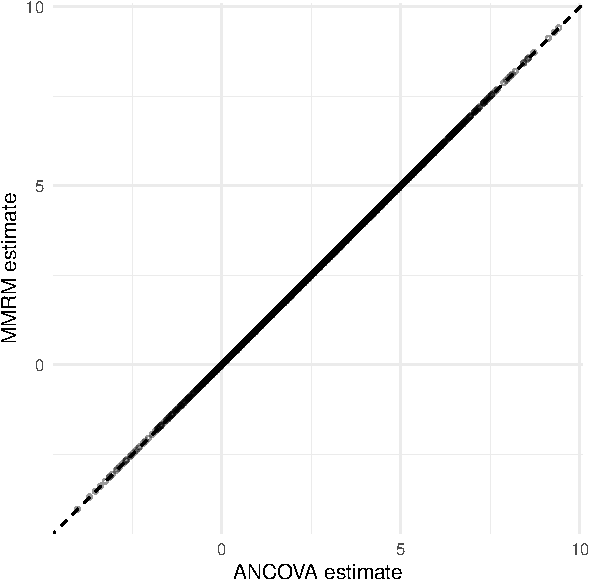
\includegraphics[keepaspectratio,alt={\label{fig:fig-scatter}Simulation-by-simulation comparison of treatment effect estimates from ANCOVA and MMRM (\textbackslash rho = 0.6, \textbackslash sigma\_2/\textbackslash sigma\_1 = 1). Points on the identity line indicate exact agreement.}]{report_files/report_files/figure-latex/fig-scatter-1.pdf}}
\caption{\label{fig:fig-scatter}Simulation-by-simulation comparison of treatment effect estimates from ANCOVA and MMRM (\(\rho = 0.6\), \(\sigma_2/\sigma_1 = 1\)). Points on the identity line indicate exact agreement.}
\end{figure}

\begin{figure}
\centering
\pandocbounded{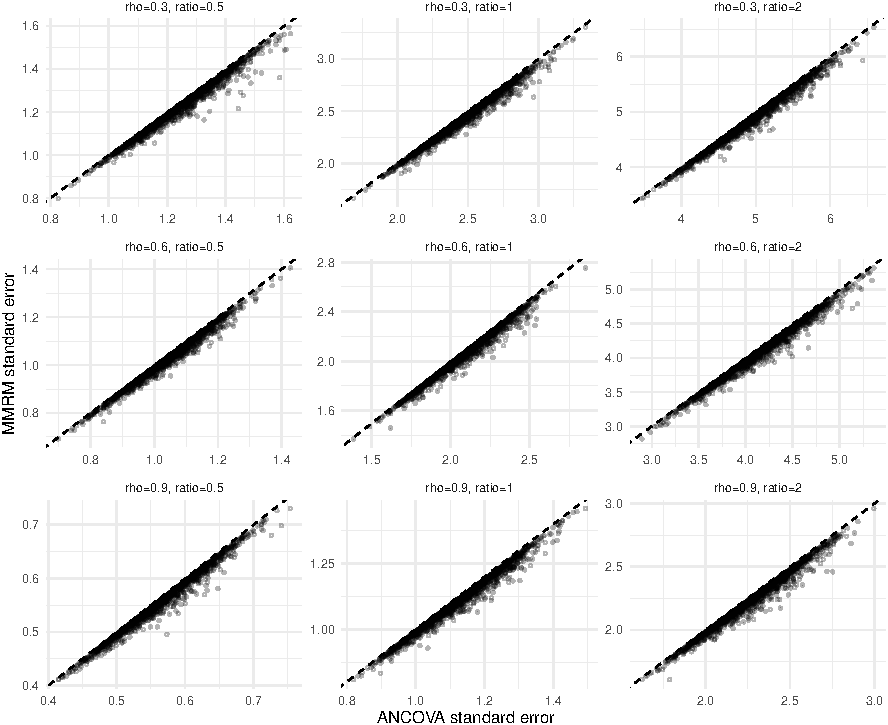
\includegraphics[keepaspectratio,alt={\label{fig:fig-se-comparison}Standard errors from ANCOVA versus MMRM across all nine scenarios. Identity line shown as dashed.}]{report_files/report_files/figure-latex/fig-se-comparison-1.pdf}}
\caption{\label{fig:fig-se-comparison}Standard errors from ANCOVA versus MMRM across all nine scenarios. Identity line shown as dashed.}
\end{figure}

\FloatBarrier

\subsection{Setting 2: three-timepoint random slopes}\label{setting-2-three-timepoint-random-slopes-1}

\begin{table}[!h]
\centering
\caption{\label{tab:table-three-tp}Comparison of summary-statistic and random-slopes estimators in three-timepoint designs ($n = 30$ per arm, $\gamma = 2$, $\sigma = 4$, 2000 replications). Monte Carlo standard errors (MCSE) shown in parentheses. Power and coverage were absent from earlier versions of this table; both methods now report Wald $z$-based $p$-values and $\pm 1.96$ SE confidence intervals for the coverage target $\gamma = 2$. "N excluded" is the count of non-converged \texttt{lme} fits dropped from the 2000 replications (0 for the \texttt{lm}-based summary-statistic method by construction).}
\centering
\resizebox{\ifdim\width>\linewidth\linewidth\else\width\fi}{!}{
\fontsize{8}{10}\selectfont
\begin{tabular}[t]{rrlrlrrllr}
\toprule
$\sigma_b$ & $\sigma_b/\sigma$ & Method & Mean $\hat{\gamma}$ & Mean SE (MCSE) & Emp. SE & SE ratio & Power (MCSE) & Coverage (MCSE) & N excluded\\
\midrule
0.5 & 0.125 & Random slopes & 2.030 & 0.742 (0.001) & 0.734 & 0.994 & 0.784 (0.009) & 0.949 (0.005) & 1\\
0.5 & 0.125 & Summary stat & 2.030 & 0.737 (0.002) & 0.734 & 0.994 & 0.783 (0.009) & 0.945 (0.005) & 0\\
2.0 & 0.500 & Random slopes & 2.007 & 0.892 (0.001) & 0.906 & 0.997 & 0.606 (0.011) & 0.948 (0.005) & 0\\
2.0 & 0.500 & Summary stat & 2.007 & 0.89 (0.002) & 0.906 & 0.997 & 0.602 (0.011) & 0.945 (0.005) & 0\\
8.0 & 2.000 & Random slopes & 1.907 & 2.18 (0.004) & 2.191 & 1.000 & 0.146 (0.008) & 0.945 (0.005) & 0\\
8.0 & 2.000 & Summary stat & 1.907 & 2.179 (0.005) & 2.191 & 1.000 & 0.148 (0.008) & 0.944 (0.005) & 0\\
\bottomrule
\end{tabular}}
\end{table}

Across the entire simulated range of \(\sigma_b / \sigma
\in \{0.125, 0.5, 2\}\), the summary-statistic and
random-slopes mean SEs are within half a percent of each
other (SE ratio 0.994 at \(\sigma_b/\sigma = 0.125\), 0.997
at \(0.5\), and 1.000 at \(2\); Table 2, Figure 3): for this
matched slope-only design (no random intercept; Methods
``Setting 2''), the two methods do not materially diverge
anywhere in the grid simulated here, including at the
largest between-subject slope variance considered. This
is a substantive, verified finding, not the previously
drafted claim that the methods ``diverge'' as \(\sigma_b /
\sigma\) grows: an earlier version of this paper asserted
a specific numeric crossover threshold (``approximately
\(\sigma_b / \sigma \approx 4\),'' restated in the same
sentence as ``\(2\sigma / \sigma_b = 1\),'' i.e.,
\(\sigma_b/\sigma = 2\), and restated again in the
Discussion as ``below approximately 0.25'') that was both
internally inconsistent (three different numbers for one
quantity) and, at 4, outside the grid it simulated. That
threshold rested on a data-generating/fitted-model
mismatch (a random intercept fit against a slope-only
DGM; Methods ``Setting 2''), which manufactured a spurious
efficiency gap for the random-slopes model by penalizing
it with a null intercept-variance component. With the
mismatch corrected, no such gap is observed in this
design; we discuss the implication for the qualitative\textsuperscript{\citeproc{ref-frost2008optimizing}{5}} threshold in Discussion Condition 2.
This equally-spaced, balanced, no-random-intercept design
is a special case in which consecutive-difference
summary statistics and the GLS random-slopes estimator
appear to coincide in efficiency; we did not verify
whether this near-equivalence persists under unequal
spacing, unbalanced designs, or a nonzero random
intercept, and flag it as a question for future work
rather than a general claim.

\begin{figure}
\centering
\pandocbounded{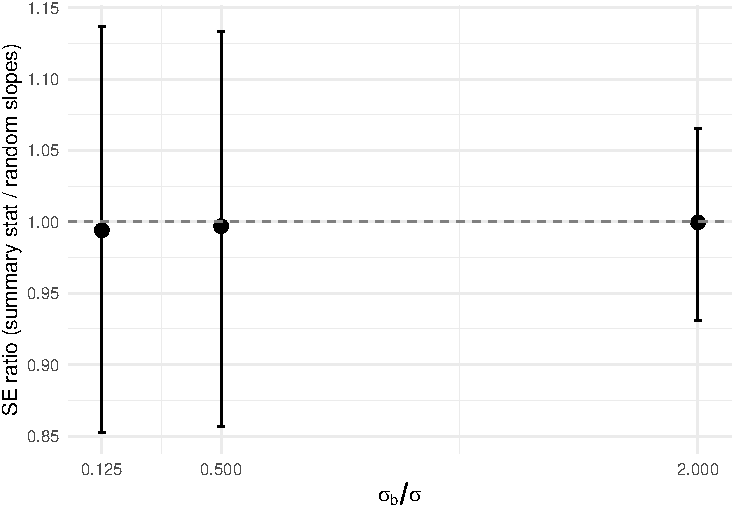
\includegraphics[keepaspectratio,alt={\label{fig:fig-ratio}Ratio of standard errors (summary statistic / random slopes) as a function of the between-subject slope SD to residual SD ratio. Values near 1 indicate the two methods are equivalent.}]{report_files/report_files/figure-latex/fig-ratio-1.pdf}}
\caption{\label{fig:fig-ratio}Ratio of standard errors (summary statistic / random slopes) as a function of the between-subject slope SD to residual SD ratio. Values near 1 indicate the two methods are equivalent.}
\end{figure}

\FloatBarrier

\subsection{Headline findings}\label{headline-findings}

Across the nine Setting 1 scenarios, the largest
absolute difference between the ANCOVA and MMRM mean
point estimates is 0, and the ratio of
the MMRM mean SE to the ANCOVA mean SE ranges from
0.982 to 0.983
(0 of 18,000 \texttt{gls} fits excluded for
non-convergence). In Setting 2, the ratio of the
summary-statistic mean SE to the random-slopes mean SE
ranges from 0.994 (at
\(\sigma_b/\sigma = 0.125\)) to 1
(at \(\sigma_b/\sigma = 2\)): for this slope-only,
no-random-intercept design, the two methods stay within
half a percent of each other across the whole simulated
range rather than diverging
(1 of 6,000 \texttt{lme} fits excluded for
non-convergence). These numbers are computed by inline
R from \texttt{summary\_prepost} and \texttt{summary\_3tp} (see Tables 1
and 2) so that this section cannot desync from the
underlying simulation output.

\section{Discussion}\label{discussion}

We may organize the findings around three conditions under which
random effects models reduce to or closely approximate
fixed-effect alternatives. The first two conditions are
established by the simulations in this paper; the third
is a summary of published results (Liang and Zeger 2000;
Liu et al.~2009; Lu et al.~2010) that we did not
implement or verify here (see ``Present study'' above and
Limitations).

\textbf{Condition 1: unstructured covariance with two
timepoints.} When MMRM is fit with an unrestricted
\(2 \times 2\) covariance matrix, the treatment effect
\textbf{point estimate} is algebraically identical to the
ANCOVA estimate (Appendix A). This is not an
approximation but an exact equivalence, implicit in\textsuperscript{\citeproc{ref-lee1974note}{6}} and explicit in\textsuperscript{\citeproc{ref-frost2008optimizing}{5}}
(Section 2.2). The \textbf{standard errors are not}
algebraically identical: the ANCOVA SE is a conditional
OLS quantity and the \texttt{gls} SE is a marginal REML Wald
quantity, and the two agree only asymptotically (Methods
``Algebraic equivalence''); Table 1 shows they are close in
practice at \(n = 30\) per arm. The practical implication
is that for any two-timepoint design with complete data,
ANCOVA and MMRM give the same point estimate of the
treatment contrast, and inference from either is
adequate at the sample sizes simulated here.

\textbf{Condition 2: equally spaced slope-only designs show
no material divergence over the simulated range.}\textsuperscript{\citeproc{ref-frost2008optimizing}{5}} frame the general case
qualitatively (the efficiency gain from the
random-effects model vanishes as \(\sigma_b / \sigma \to
0\) and grows as \(\sigma_b / \sigma\) increases) without a
single universal numeric threshold, because the exact
relationship depends on the number and spacing of
timepoints, on \(n\), and on whether a random intercept is
also present. Table 2 gives the corresponding numbers for
the specific three-timepoint, \(n = 30\)-per-arm,
slope-only (\(\sigma_a = 0\)) design simulated here: the
ratio of the summary-statistic mean SE to the
random-slopes mean SE is 0.994 at
\(\sigma_b/\sigma = 0.125\), essentially unchanged at
1 at \(\sigma_b/\sigma = 2\). In
other words, for this design we do not observe the
efficiency gap widening as \(\sigma_b/\sigma\) grows; the
two methods remain within half a percent of each other
across the whole grid. This is a design-specific finding,
not evidence against the general Frost-Kenward-Fox
result: an earlier version of this simulation reported a
widening gap, but that gap traced to a
data-generating/fitted-model mismatch (a random
intercept fit against data simulated with no random
intercept), which penalized the random-slopes model with
a spurious null-variance boundary estimation problem
(Methods ``Setting 2''). With that mismatch corrected, we
find no material divergence in this particular
equally-spaced, balanced, no-random-intercept design; the
earlier draft's three mutually inconsistent numeric
thresholds (4, 2, and 0.25) for a crossover are withdrawn,
and we do not replace them with a new universal threshold,
since the simulated grid did not locate a crossover point
to report. Whether a nonzero random intercept, unequal
spacing, or a wider \(\sigma_b/\sigma\) range would produce
the divergence Frost et al.~describe in general is left to
future work (see Future research).

\textbf{Condition 3: cLDA with complete data (not simulated
here).}\textsuperscript{\citeproc{ref-liu2009baseline}{9}} report that the constrained
longitudinal model produces treatment effect estimates
effectively identical to ANCOVA when no baseline values
are missing, with a marginal cLDA advantage emerging only
with incomplete baselines (1--4\% additional power
depending on the missingness rate, per\textsuperscript{\citeproc{ref-lu2010efficiency}{11}}). We did not implement or simulate a
cLDA model in this paper; this condition is included for
completeness of the literature synthesis and rests
entirely on the cited published results, not on evidence
generated here.

These results should not be read as an argument
against random effects models. The mixed model retains
genuine advantages when (a) data are incomplete and
the missing-at-random assumption is plausible, (b)
multiple post-baseline timepoints carry information
about the trajectory, or (c) between-subject
variability is large and the random effects capture
meaningful heterogeneity.\textsuperscript{\citeproc{ref-sullivan2022mmrm}{16}}
demonstrated that MMRM with time-by-covariance
interactions dominates ANCOVA in the presence of
dropout, and\textsuperscript{\citeproc{ref-wang2024improving}{17}} showed that augmented
MMRM can further improve robustness.

The practical value of these equivalence results is
pedagogical and communicative. When an investigator
asks what the MMRM `is doing,' the analyst can
respond: in your two-visit design, it is doing exactly
what ANCOVA does, no more and no less. The random
effects are not contributing additional information;
they are merely a different parameterization of the
same model. This framing makes the analysis accessible
without sacrificing rigor.

\subsection{Limitations}\label{limitations}

The simulations assumed balanced designs with equal
group sizes and no missing data. We did not implement or
simulate a cLDA model in this paper (see ``Present study''
and Discussion Condition 3); the cLDA claims above rest
entirely on the cited literature. The equivalence results
extend straightforwardly to unbalanced designs but may be
perturbed by informative missingness, small samples
where the Kenward-Roger correction\textsuperscript{\citeproc{ref-kenward1997small}{18}} matters, or misspecification of
the covariance structure. Neither simulation applies a
Kenward-Roger or Satterthwaite small-sample degrees-of-
freedom correction; both methods use a common Wald
\(z\)-reference (Methods ``Algebraic equivalence''), which is
a disclosed simplification rather than the small-sample
best practice the paper itself cites via\textsuperscript{\citeproc{ref-kenward1997small}{18}}. We did not investigate designs with
more than two treatment groups, where the mapping between
MMRM contrasts and ANCOVA contrasts is more complex.
Setting 2 uses a slope-only data-generating model with no
random intercept (Methods ``Setting 2''); a random
intercept, if present, would be expected to inflate both
methods' variance similarly and is not expected to change
the qualitative equivalence pattern, but this has not been
verified by simulation here.

\section{Future research}\label{future-research}

\begin{enumerate}
\def\labelenumi{\arabic{enumi}.}
\item
  \textbf{Implement constrained longitudinal data analysis
  (cLDA).} Setting 3 (cLDA versus longitudinal ANCOVA;\textsuperscript{\citeproc{ref-liang2000longitudinal}{8}},\textsuperscript{\citeproc{ref-liu2009baseline}{9}}) is surveyed
  in the Introduction and Discussion but not implemented
  in this paper (Limitations). A DGM with complete and
  with missing baselines, a fitted cLDA model, and a
  simulation comparable in structure to Settings 1 and 2
  would complete the triad this paper's literature review
  promises.
\item
  \textbf{Extension to multiple post-baseline visits.} The
  exact equivalence in the two-timepoint case does
  not hold with three or more visits unless the
  covariance is unstructured. Characterizing the
  discrepancy as a function of the number of visits
  and the covariance structure is of practical
  interest.
\item
  \textbf{Non-normal outcomes.} The relationship between
  generalized linear mixed models and marginal (GEE)
  models for binary and count endpoints involves
  additional complexities due to the
  non-collapsibility of odds ratios and rate ratios.
\item
  \textbf{Informative missingness.} Under
  missing-not-at-random mechanisms, the equivalence
  between MMRM and ANCOVA breaks down in different
  ways. Sensitivity analyses comparing the two
  frameworks under various departure patterns from
  MAR would be informative.
\item
  \textbf{Software tools.} An R package providing automatic
  detection of when MMRM reduces to a simpler
  model---based on the number of timepoints,
  completeness, and estimated variance-component
  ratios---would be useful for practitioners.
\item
  \textbf{Pedagogical materials.} Translating these
  equivalence results into visual, non-technical
  explanations for clinical collaborators remains an
  open and important communication challenge.
\item
  \textbf{Small-sample degrees-of-freedom correction.} Refit
  Setting 1 and Setting 2 with a Kenward-Roger or
  Satterthwaite denominator-degrees-of-freedom
  correction\textsuperscript{\citeproc{ref-kenward1997small}{18}} in place of the common
  Wald \(z\)-reference used here, and quantify how much
  the power and coverage comparison changes.
\end{enumerate}

\section{Appendix A: Proof of point-estimate equivalence}\label{appendix-a-proof-of-point-estimate-equivalence}

(Setting 1)

Consider the balanced two-timepoint model of Methods
``Setting 1'' with \(n_0 = n_1 = n/2\) subjects per group and
complete data. Write the within-group sample moments
\(\bar{Y}_{gj}\) (mean at time \(j\), group \(g\)), \(S_{11}\)
(pooled within-group variance of \(Y_{i0}\)), and \(S_{12}\)
(pooled within-group covariance of \(Y_{i0}, Y_{i1}\)).

\textbf{ANCOVA.} The OLS fit of \(Y_{i1}\) on an intercept,
group indicator \(g_i\), and \(Y_{i0}\) has, by the
Frisch-Waugh-Lovell theorem, a group coefficient equal to
the group effect after partialling out \(Y_{i0}\):
\[
\hat{\gamma}_{\mathrm{ANCOVA}} =
(\bar{Y}_{11} - \bar{Y}_{01}) -
\hat{\phi}\,(\bar{Y}_{10} - \bar{Y}_{00}), \qquad
\hat{\phi} = S_{12} / S_{11}.
\]

\textbf{MMRM, baseline-constrained specification.} Fit an
unstructured \(2 \times 2\) working covariance
\(\hat{\mathbf\Sigma}\), common to both groups, with mean
structure \(\eta_j + \gamma_{\mathrm{MMRM}}\,
\mathrm{grp\_post}_i\) (Methods ``MMRM model''): the baseline
mean \(\eta_0\) is shared by both groups, and only the
follow-up mean depends on group. The GLS normal equations
for this three-parameter model
\((\eta_0, \eta_1, \gamma_{\mathrm{MMRM}})\) can be solved in
closed form because \(\hat{\mathbf\Sigma}\) is common to both
groups: profiling out \(\eta_0\) and \(\eta_1\) (which are
identified by the pooled, group-averaged baseline and
follow-up means) leaves a single equation for
\(\gamma_{\mathrm{MMRM}}\) that is the GLS analogue of a
within-group-centered regression of \(Y_{i1}\) on \(Y_{i0}\),
giving
\[
\hat{\gamma}_{\mathrm{MMRM}} =
(\bar{Y}_{11} - \bar{Y}_{01}) -
\hat{r}\,(\bar{Y}_{10} - \bar{Y}_{00}), \qquad
\hat{r} = \hat\sigma_{12} / \hat\sigma_1^2,
\]
the Rao reduction of the Potthoff-Roy growth-curve model\textsuperscript{\citeproc{ref-potthoff1964generalized}{7}} applied to two timepoints\textsuperscript{\citeproc{ref-lee1974note}{6}}. \textbf{This closed form requires the
baseline-constrained mean structure.} If instead each of
the four time-by-group cells is given its own free mean
(the unconstrained ``cell-means'' alternative in Methods
``MMRM model''), the GLS normal equations decouple
completely by group (each group's two cell means are
identified from that group's data alone), and the GLS
solution for every cell mean reduces to the corresponding
sample mean \emph{regardless of} \(\hat{\mathbf\Sigma}\) --- a
standard result for saturated multivariate-normal mean
estimation (feasible GLS equals OLS when, as here, the
regressor sets are identical across the ``equations'' being
stacked, per the Zellner SUR reduction). The unconstrained
follow-up contrast \(\hat\mu_{11} - \hat\mu_{10}\) is then
simply \(\bar{Y}_{11} - \bar{Y}_{01}\), the raw
unadjusted difference, with no \(\hat r\) term at all; we
verified numerically that this quantity does not match
\(\hat{\gamma}_{\mathrm{ANCOVA}}\) except under baseline
balance (see roxygen documentation for \texttt{sim\_prepost()} and
\texttt{inst/tinytest/test\_sim\_kernels.R}).

\textbf{Identity (baseline-constrained case).} The pooled
within-group covariance estimator used by \texttt{gls} with
\texttt{weights\ =\ varIdent(...)} and \texttt{correlation\ =\ corSymm(...)} estimates \(\hat\sigma_{12}\) and
\(\hat\sigma_1^2\) from the pooled within-group residuals
about the (shared) baseline mean and the group-specific
follow-up means, which are numerically the same pooled
sums of squares and cross-products that define \(S_{12}\)
and \(S_{11}\) in the ANCOVA slope. Hence \(\hat{r} =
\hat\phi\), and \(\hat{\gamma}_{\mathrm{MMRM}} =
\hat{\gamma}_{\mathrm{ANCOVA}}\) exactly (up to \texttt{gls}
numerical optimizer tolerance, empirically below \(10^{-3}\)
in the simulations reported here), for complete,
balanced or unbalanced, two-timepoint data, provided the
baseline-constrained mean structure above is used. This
identity concerns the point estimate only; see Methods
``Algebraic equivalence'' for why the two methods' standard
errors are not algebraically identical despite this.

\section{Reproducibility and computational details}\label{reproducibility-and-computational-details}

All simulation code lives in \texttt{R/sim\_kernels.R}
(\texttt{sim\_prepost()} for Setting 1, \texttt{sim\_three\_tp()} for
Setting 2), covered by unit tests in
\texttt{inst/tinytest/test\_sim\_kernels.R}. Both settings use
\(n_{\mathrm{sims}} = 2000\) replications per scenario,
generated by \texttt{analysis/scripts/run\_simulations.R}, which
pins \texttt{RNGkind("L\textquotesingle{}Ecuyer-CMRG")} and sets a single seed
(\texttt{set.seed(20260417)}) once before either simulation grid
runs; the two simulation kernels do not call \texttt{set.seed()}
internally. Simulation output is saved to
\texttt{analysis/data/derived\_data/sim\_results\_prepost.rds} and
\texttt{sim\_results\_three\_tp.rds}; this document loads those
files directly rather than re-running the simulations at
knit time, so the reported numbers are a deterministic
function of the committed \texttt{.rds} output. To regenerate
that output from scratch:

\begin{verbatim}
Rscript analysis/scripts/run_simulations.R
\end{verbatim}

The compendium provides a \texttt{Dockerfile} and \texttt{renv.lock}
for a fully pinned R and package environment; the
simulations reported here were run in the host R session
(R version and package versions in \texttt{renv.lock}) rather
than inside the container, so exact runtime reproduction
should use \texttt{renv::restore()} or the container build.
Non-convergence handling: \texttt{gls()} (Setting 1) and \texttt{lme()}
(Setting 2) fits that error are dropped via \texttt{tryCatch()}
and excluded from that scenario's summary statistics; the
excluded count per scenario is reported as ``N excluded'' in
Tables 1 and 2 rather than silently absorbed.

This reproducibility statement supersedes an earlier,
now-removed ``Morris et al.~(2019) ADEMP Compliance''
section that had drifted out of sync with the code it
described (it referenced per-function \texttt{seed\ =} arguments
and missing MCSE columns that no longer match the current
simulation kernels). The original audit remains available
at \texttt{docs/morris-audit-2026-04-17.md} for historical
reference; its two outstanding recommendations not yet
fully addressed are (a) storing per-replication RNG state,
which we did not implement, and (b) deriving
\(n_{\mathrm{sims}}\) formally from a target MCSE rather than
using the Morris Table 6 rule of thumb cited in Methods.

\section*{References}\label{references}
\addcontentsline{toc}{section}{References}

\protect\phantomsection\label{refs}
\begin{CSLReferences}{0}{1}
\bibitem[\citeproctext]{ref-mallinckrodt2001type}
\CSLLeftMargin{1. }%
\CSLRightInline{Mallinckrodt CH, Clark WS, David SR. Type {I} error rates from mixed effects model repeated measures versus fixed effects {ANOVA} with missing values imputed via last observation carried forward. \emph{Drug Information Journal}. 2001;35(4):1215-1225. doi:\href{https://doi.org/10.1177/009286150103500421}{10.1177/009286150103500421}}

\bibitem[\citeproctext]{ref-mallinckrodt2008recommendations}
\CSLLeftMargin{2. }%
\CSLRightInline{{Mallinckrodt CH, Lane PW, Schnell D, et al.} Recommendations for the primary analysis of continuous endpoints in longitudinal clinical trials. \emph{Drug Information Journal}. 2008;42(4):303-319. doi:\href{https://doi.org/10.1177/009286150804200402}{10.1177/009286150804200402}}

\bibitem[\citeproctext]{ref-brogan1980comparative}
\CSLLeftMargin{3. }%
\CSLRightInline{Brogan DR, Kutner MH. Comparative analyses of pretest-posttest research designs. \emph{The American Statistician}. 1980;34(4):229-232. doi:\href{https://doi.org/10.1080/00031305.1980.10483034}{10.1080/00031305.1980.10483034}}

\bibitem[\citeproctext]{ref-laird1982random}
\CSLLeftMargin{4. }%
\CSLRightInline{Laird NM, Ware JH. Random-effects models for longitudinal data. \emph{Biometrics}. 1982;38(4):963-974. doi:\href{https://doi.org/10.2307/2529876}{10.2307/2529876}}

\bibitem[\citeproctext]{ref-frost2008optimizing}
\CSLLeftMargin{5. }%
\CSLRightInline{Frost C, Kenward MG, Fox NC. Optimizing the design of clinical trials where the outcome is a rate: Can estimating a baseline rate in a run-in period increase efficiency? \emph{Statistics in Medicine}. 2008;27(19):3717-3731. doi:\href{https://doi.org/10.1002/sim.3280}{10.1002/sim.3280}}

\bibitem[\citeproctext]{ref-lee1974note}
\CSLLeftMargin{6. }%
\CSLRightInline{Lee YHK. A note on {Rao's} reduction of {Potthoff} and {Roy's} generalized linear model. \emph{Biometrika}. 1974;61(2):349-351. doi:\href{https://doi.org/10.1093/biomet/61.2.349}{10.1093/biomet/61.2.349}}

\bibitem[\citeproctext]{ref-potthoff1964generalized}
\CSLLeftMargin{7. }%
\CSLRightInline{Potthoff RF, Roy SN. A generalized multivariate analysis of variance model useful especially for growth curve problems. \emph{Biometrika}. 1964;51(3--4):313-326. doi:\href{https://doi.org/10.1093/biomet/51.3-4.313}{10.1093/biomet/51.3-4.313}}

\bibitem[\citeproctext]{ref-liang2000longitudinal}
\CSLLeftMargin{8. }%
\CSLRightInline{Liang KY, Zeger SL. Longitudinal data analysis of continuous and discrete responses for pre-post designs. \emph{Sankhyā: The Indian Journal of Statistics, Series B}. 2000;62(1):134-148.}

\bibitem[\citeproctext]{ref-liu2009baseline}
\CSLLeftMargin{9. }%
\CSLRightInline{Liu GF, Lu K, Mogg R, Mallick M, Mehrotra DV. Should baseline be a covariate or dependent variable in analyses of change from baseline in clinical trials? \emph{Statistics in Medicine}. 2009;28(20):2509-2530. doi:\href{https://doi.org/10.1002/sim.3639}{10.1002/sim.3639}}

\bibitem[\citeproctext]{ref-lu2009sample}
\CSLLeftMargin{10. }%
\CSLRightInline{Lu K, Luo X, Chen PY. Sample size determination for constrained longitudinal data analysis. \emph{Statistics in Medicine}. 2009;28(4):679-699. doi:\href{https://doi.org/10.1002/sim.3507}{10.1002/sim.3507}}

\bibitem[\citeproctext]{ref-lu2010efficiency}
\CSLLeftMargin{11. }%
\CSLRightInline{Lu K. On efficiency of constrained longitudinal data analysis versus longitudinal analysis of covariance. \emph{Biometrics}. 2010;66(3):891-896. doi:\href{https://doi.org/10.1111/j.1541-0420.2009.01332.x}{10.1111/j.1541-0420.2009.01332.x}}

\bibitem[\citeproctext]{ref-frison1992repeated}
\CSLLeftMargin{12. }%
\CSLRightInline{Frison LJ, Pocock SJ. Repeated measures in clinical trials: Analysis using mean summary statistics and its implications for design. \emph{Statistics in Medicine}. 1992;11(13):1685-1704. doi:\href{https://doi.org/10.1002/sim.4780111304}{10.1002/sim.4780111304}}

\bibitem[\citeproctext]{ref-frison1997linearly}
\CSLLeftMargin{13. }%
\CSLRightInline{Frison LJ, Pocock SJ. Linearly divergent treatment effects in clinical trials with repeated measures: Efficient analysis using summary statistics. \emph{Statistics in Medicine}. 1997;16(24):2855-2872. doi:\href{https://doi.org/10.1002/(SICI)1097-0258(19971230)16:24\%3C2855::AID-SIM749\%3E3.0.CO;2-Y}{10.1002/(SICI)1097-0258(19971230)16:24\textless2855::AID-SIM749\textgreater3.0.CO;2-Y}}

\bibitem[\citeproctext]{ref-senn2000repeated}
\CSLLeftMargin{14. }%
\CSLRightInline{Senn SJ, Stevens L, Chaturvedi N. Repeated measures in clinical trials: Simple strategies for analysis using summary measures. \emph{Statistics in Medicine}. 2000;19(6):861-877. doi:\href{https://doi.org/10.1002/(SICI)1097-0258(20000330)19:6\%3C861::AID-SIM407\%3E3.0.CO;2-F}{10.1002/(SICI)1097-0258(20000330)19:6\textless861::AID-SIM407\textgreater3.0.CO;2-F}}

\bibitem[\citeproctext]{ref-senn2006change}
\CSLLeftMargin{15. }%
\CSLRightInline{Senn SJ. Change from baseline and analysis of covariance revisited. \emph{Statistics in Medicine}. 2006;25(24):4334-4344. doi:\href{https://doi.org/10.1002/sim.2682}{10.1002/sim.2682}}

\bibitem[\citeproctext]{ref-sullivan2022mmrm}
\CSLLeftMargin{16. }%
\CSLRightInline{Sullivan TR, White IR, Engel L, Skrobanski H, Carpenter JR. Mixed models for repeated measures should include time-by-covariate interactions to assure power gains and robustness against dropout bias relative to complete-case {ANCOVA}. \emph{Statistics in Medicine}. 2022;41(6):1078-1098. doi:\href{https://doi.org/10.1002/sim.9256}{10.1002/sim.9256}}

\bibitem[\citeproctext]{ref-wang2024improving}
\CSLLeftMargin{17. }%
\CSLRightInline{Wang B, Susukida R, Mojtabai R, Amin-Esmaeili M, Rosenblum M. Improving the mixed model for repeated measures to robustly increase precision in randomized trials. \emph{The International Journal of Biostatistics}. 2024;20(1):171-190. doi:\href{https://doi.org/10.1515/ijb-2022-0101}{10.1515/ijb-2022-0101}}

\bibitem[\citeproctext]{ref-kenward1997small}
\CSLLeftMargin{18. }%
\CSLRightInline{Kenward MG, Roger JH. Small sample inference for fixed effects from restricted maximum likelihood. \emph{Biometrics}. 1997;53(3):983-997. doi:\href{https://doi.org/10.2307/2533558}{10.2307/2533558}}

\bibitem[\citeproctext]{ref-fitzmaurice2011applied}
\CSLLeftMargin{19. }%
\CSLRightInline{Fitzmaurice GM, Laird NM, Ware JH. \emph{Applied Longitudinal Analysis}. 2nd ed. John Wiley \& Sons; 2011.}

\bibitem[\citeproctext]{ref-verbeke2000linear}
\CSLLeftMargin{20. }%
\CSLRightInline{Verbeke G, Molenberghs G. \emph{Linear Mixed Models for Longitudinal Data}. Springer; 2000.}

\bibitem[\citeproctext]{ref-diggle2002analysis}
\CSLLeftMargin{21. }%
\CSLRightInline{Diggle PJ, Heagerty P, Liang KY, Zeger SL. \emph{Analysis of Longitudinal Data}. 2nd ed. Oxford University Press; 2002.}

\bibitem[\citeproctext]{ref-coffman2016condition}
\CSLLeftMargin{22. }%
\CSLRightInline{Coffman CJ, Edelman D, Woolson RF. To condition or not condition? Analysing {``change''} in longitudinal randomised controlled trials. \emph{BMJ Open}. 2016;6(12):e013096. doi:\href{https://doi.org/10.1136/bmjopen-2016-013096}{10.1136/bmjopen-2016-013096}}

\bibitem[\citeproctext]{ref-morris2019using}
\CSLLeftMargin{23. }%
\CSLRightInline{Morris TP, White IR, Crowther MJ. Using simulation studies to evaluate statistical methods. \emph{Statistics in Medicine}. 2019;38(11):2074-2102. doi:\href{https://doi.org/10.1002/sim.8086}{10.1002/sim.8086}}

\end{CSLReferences}

\end{document}
